\documentclass[conference]{IEEEtran}
\usepackage{blindtext, graphicx}
\usepackage[cmex10]{amsmath}
\usepackage[backend=biber]{biblatex}
\addbibresource{ref.bib}

\begin{document}

\title{Predicting Hospital Readmission Rate of Diabetic Patients}


% author names and affiliations
% use a multiple column layout for up to three different
% affiliations
\author{\IEEEauthorblockN{Ashish Kumar}
\IEEEauthorblockA{Department of Mining Engineering\\
McGill University\\
ashish.kumar@mail.mcgill.ca}
\and
\IEEEauthorblockN{Charlie Bloomfield}
\IEEEauthorblockA{School of Computer Science\\
McGill University\\
charles.bloomfield@mail.mcgill.ca}
\and
\IEEEauthorblockN{Jonathan Campbell}
\IEEEauthorblockA{School of Computer Science\\
McGill University\\
jonathan.campbell@mcgill.ca}}

\maketitle

\begin{abstract}

Using an existing dataset of patient-hospital encounters, we present methodology for predicting the readmission of diabetic patients based on selected features of the encounters. An existing dataset of encounters from 130 U.S. hospitals was used~\cite{dataset-2014} and pre-processing of this dataset is discussed with respect to problems of class imbalances and missing data. The best performance was obtained using the Support Vector Machines algorithm with a precision value of 61\%.

\end{abstract}

% An example of a double column floating figure using two subfigures.
% (The subfig.sty package must be loaded for this to work.)
% The subfigure \label commands are set within each subfloat command, the
% \label for the overall figure must come after \caption.
% \hfil must be used as a separator to get equal spacing.
% The subfigure.sty package works much the same way, except \subfigure is
% used instead of \subfloat.
%
%\begin{figure*}[!t]
%\centerline{\subfloat[Case I]\includegraphics[width=2.5in]{subfigcase1}%
%\label{fig_first_case}}
%\hfil
%\subfloat[Case II]{\includegraphics[width=2.5in]{subfigcase2}%
%\label{fig_second_case}}}
%\caption{Simulation results}
%\label{fig_sim}
%\end{figure*}

% An example of a floating table. Note that, for IEEE style tables, the 
% \caption command should come BEFORE the table. Table text will default to
% \footnotesize as IEEE normally uses this smaller font for tables.
% The \label must come after \caption as always.
%
%\begin{table}[!t]
%% increase table row spacing, adjust to taste
%\renewcommand{\arraystretch}{1.3}
% if using array.sty, it might be a good idea to tweak the value of
% \extrarowheight as needed to properly center the text within the cells
%\caption{An Example of a Table}
%\label{table_example}
%\centering
%% Some packages, such as MDW tools, offer better commands for making tables
%% than the plain LaTeX2e tabular which is used here.
%\begin{tabular}{|c||c|}
%\hline
%One & Two\\
%\hline
%Three & Four\\
%\hline
%\end{tabular}
%\end{table}

\section{Introduction}

Diabetes affects 336 million people worldwide and is predicted to increase to 552 million in 2030~\cite{estimates-2011}. Prediction of relevant factors resulting in readmission of diabetic patients is very important to reduce the large physical and finanical costs associated with readmission. This paper deals with the prediction of readmission of diabetic patients using a machine learning approach on a pre-existing dataset. We describe related research with said dataset in section 2, followed by a brief description of the dataset in section 3. Due to particularities with the dataset, several data pre-processing methods were performed and are discussed in section 4, followed by an explanation of the performance measurement criteria used in the project in section 5. We continue with brief descriptions of machine learning algorithms used, including baseline methods, with some focus on methods known to perform better on the dataset. The paper concludes with presentation and discussion of results and future work.

\subsection{Target Prediction Task}

As mentioned above, the goal of this paper is to predict the readmission of diabetic patients based on various features recorded during their hospital visits. There are three target classes: readmitted before 30 days (class 0), after 30 days (class 1), or not readmitted at all (class 2).

\section{Related Work}

Diabetes or “diabetes mellitus” is a metabolic disorder characterized by hyperglycemia and disturbance of metabolism of fat protein and carbohydrates, caused by imperfections of insulin secretion or functioning~\cite{worldhealthorganization-2015}. Morbidity of patients in hospitals is significantly determined by the management of hyperglycemia in the hospitalized patients~\cite{hyperglycemia-2002, unrecognizeddiabetes-1998}. Readmission of patients to hospitals impacts the economy and quality of healthcare services. In terms of cost, readmission of patients cost the United States \$41.3 billion in 2011~\cite{estimates-2011}, out of which unchecked diabetes accounted for 23,700 readmissions at a cost of \$251 million~\cite{sas-2015}. Rising readmission rates have prompted the Centers for Medicare \& Medicaid Services (CMS) to introduce measures to curb the problem~\cite{readmissionreduction-2015}.

The impact of HbA1c measurement on hospital readmission rates was studied with the same dataset we are using using a multivariate logistic regression algorithm~\cite{hba1c-2014}. Although the research showed the importance of this feature, a study of other relevant features was excluded. Another paper used a commercial Support Vector Machine algorithm (SAS Enterprise Miner) on the same dataset and obtained an accuracy of 63.7\%~\cite{sas-2015}, but the handling of missing data was not properly managed and medical speciality of the attending doctor was removed, which is an important feature in deciding the outcome of the medical services rendered and eventually the readmission prediction. Furthermore, the measurement criteria used was the misclassification rate, which is unreliable due to the imbalance of target classes. The demographics of diabetic patients were predicted using the same database in another paper on the same dataset~\cite{cotha-2015}, and the authors obtained an accuracy of 53.3\% using an ensemble method of decision trees.

\section{Dataset Description \& Analysis}

% discuss presence of missing data, what the features are, amount, where dataset came from...

A ten-year clinical database of 130 U.S. hospitals used in a previous study of diabetic patient readmission rates was used for our target prediction task~\cite{dataset-2014, hba1c-2014}. The dataset has 101,766 instances with 49 features, including demographics, personal characteristics, information about the person's time in hospital, medical diagnoses and relevant measurements, medications administered, procedures performed, and so on. The target feature is that of readmission of said patient before 30 days, after 30 days, or not at all. The features are presented in several different types (strings, integers, ranges of integers, etc).

There is a large amount of missing data in the dataset, specifically for the weight, payer code, and medicial specialty of the attending doctor. Approaches to deal with this missing data are discussed below. Further, there is a large class imbalance in the dataset: most of the instances are of class 0 (readmitted before 30 days). Approaches to deal with this problem are also discussed below.

\section{Data Pre-processing}

% discuss categorization of data
% smote, over sampling

Medical databases in general are associated with lots of anomalies in recording, and this dataset was no different. There were two problems in particular that were encountered with this data, namely an imbalance in class examples and a large amount of missing data. We present approaches for both of these problems, as well as a brief discussion of feature selection/reduction. Several features are also in inconvenient formats for machine learning algorithms to process, so we discuss our encoding of the data as well.

\subsection{Class Imbalances}

\begin{figure}[htpb]
	\centering
	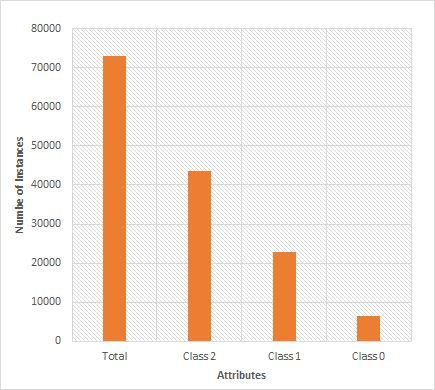
\includegraphics[width=0.4\textwidth]{class_imbalance}
	\caption{Number of instances for each class in the dataset.}
	\label{fig:class_imbalance}
\end{figure}

There was a large imbalance of classes in our dataset, leading to a poor accuracy of a classifier for the class with less instances. Figure~\ref{fig:class_imbalance} depicts the amount of data instances for each class; there is a 6.71 ratio between class 0 and class 2.

There are two general ways to solve a class imbalance problem: data-driven approaches and algorithmic approaches~\cite{purwar-2014}. One popular data-based approach using clustering is called SMOTE, which has proven to be very useful for dealing with class imbalance problem~\cite{smote-2012}. Algorithm-based approaches include a modified SVM using decision threshold adaptation~\cite{wu-2003, raskutti-2004} or variation of likelihood estimation in decision trees~\cite{weiss-2003}.

We used the SMOTE algorithm for our dataset. Class 0 examples were oversampled with a ratio of 6.71 using SMOTE technique. Class 1 instances were not oversampled as the number of instances of class 1 compared to class 0 had a ratio of 1.9. Performance of the raw vs. oversampled dataset is presented in the Results section.

Other ideas tried were to sample the same number of instances (6,000) from each class and use that to train the learners, or to merge class 1 and 2. However, neither of these results produced any improvement to precision scores.

\subsection{Missing Data}

\begin{figure}[htpb]
	\centering
	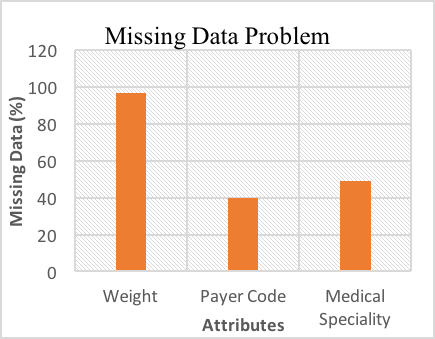
\includegraphics[width=0.4\textwidth,scale=0.7]{missing_data}
	\caption{Percentage of missing data for various features of the dataset.}
	\label{fig:missing_data}
\end{figure}

% deletion of missing data, using model-based approach to fill in values...

Missing data is a serious problem in medical databases and limits the use of machine learning algorithms on medical data. However, there are various methods available to deal with the missing data problem~\cite{imputation-96}. Treatment of the missing data should be done carefully to prevent bias introduction~\cite{gustavo-2003}. Two different methods of data imputation were attempted in this project: data deletion and data imputation. A third method, to simply categorize missing data as its own integer value (i.e. 0) was also tried.

Various model-based approaches such as Auto Class C4.5~\cite{lakshminarayan-1999}, k-nearest neighbour~\cite{gustavo-2003} etc. have also been used for data imputation in the literature. 

Figure~\ref{fig:missing_data} shows the percentage of missing data in various features of the dataset. The deletion method was applied to the weight and payer code attributes while both deletion and model-based imputation method were alternately utilized for the medical speciality attribute. Both a decision tree  and k-nearest neighbour classifier were used as models for the imputation method as was suggested from the literature. Cross-validation was used for hyperparameter optimization. The target attribute was medical speciality with 70 classes and 30891 instances of data where the medical specialty was not missing. In the end, decision trees (with depth of 11) were used for the final missing data imputation since they returned the best accuracy on the test set (51.2\%).

\subsection{Feature Selection}
% removal of certain features not relevant (as per paper), possible combination of target into 2 classes...
Feature selection is a technique that reduces the dimension of a dataset's feature space. With high-dimensional data, especially when the dimension of a feature space is as large as or greater than the number of data points in a dataset, learners tend to overfit to training data. Furthermore, it is possible that features are dependent on the values of other features, in which case they add little value to the predictions produced by learning algorithms. Effective use of feature selection techniques can mitigate these problems and improve a learner's generalization performance. 

We used two feature selection techniques with our learners: Principal Component Analysis (PCA) and Analysis of Variance (ANOVA). PCA functions by projecting the vectors in the feature space into eigenspace. In this space, it is easy to determine which components have the largest variance. These components are likely to hold the greatest predictive information, and as such they are labeled the principal components. PCA then removes a parameterized number of features to remove from the feature space and produces a transformed dataset. ANOVA performs similar feature reduction but selects the features that have the highest F-score when compared to the predicted class. It has been shown to work was a very successful technique while classifying high-dimensional datasets~cite{anova-classification}. For each algorithm, the best choice for number of features to keep can be determined with standard hyper parameter selection techniques. We used grid search for this purpose.

\subsection{Data Encoding}

\begin{figure}[htpb]
	\centering
	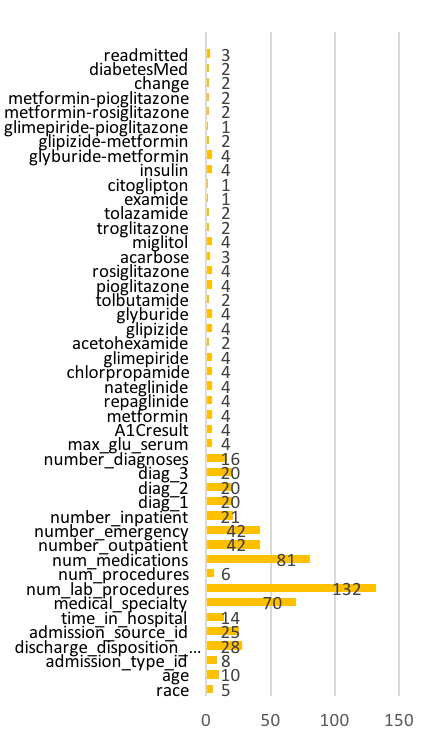
\includegraphics[width=0.4\textwidth]{dataset}
	\caption{Number of unique values for each feature in the dataset.}
	\label{fig:dataset}
\end{figure}

Values in the original dataset could take the form of strings, integer ranges, and other unpalatable types for machine learning algorithms, so were all encoded to integer values. Some features, such as medical specialty (a string in the original dataset), were converted to binary features (one feature for each possible medical specialty, with a value of 1 for the attending doctor having that medicial specialty and 0 for not having it). This conversion was done since converting said value to a categorical range of 1...n would not make sense, since it introduces an ordering to the medical specialties that has no basis in reality. Other features, such as age, were encoded using a categorical range since an ordering was already present.

Further, duplicate encounters of patients were removed from the database to satisfy the IID (independent and identically distributed) assumption of the classification algorithms.

The number of possible values for each feature is mentioned in Figure~\ref{fig:dataset} - for those that were translated to categorical ranges, the range goes from 1 to the total number of features.

\section{Performance Measurement Criteria}
% f1 score, problems with that...

Precision was used as the performance measurement criteria for the classifiers as shown in Figure~\ref{fig:precision_recall}. Since the dataset is imbalanced, measuring the accuracy of the classifier was not a feasible criterion. Also, the cost associated with classifying a patient who was readmitted as not readmitted is higher than the reverse, so precision was the better choice. Precision is given by the following equation.

\[ Precision = \frac{True Positive}{True Positive + False Positive} \]

\begin{figure}[htpb]
	\centering
	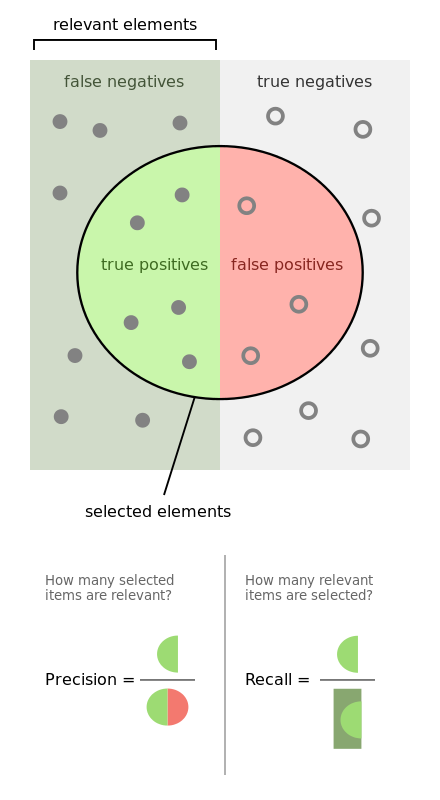
\includegraphics[width=0.25\textwidth]{precision_recall}
	\caption{Pictorial representation of precision \& recall.}
	\label{fig:precision_recall}
\end{figure}

\section{Methodology}

Several baseline learners were tried to get a sense of an average performance on the dataset. Other classifiers which have been shown to perform well in the medical literature were also attempted, including Support Vector Machines, Neural Networks and Adaboost, and are discussed in more detail.

For all algorithms, the train/test split was 66\%/33\%. The precision metric was used to rate their performance.

\subsection{Baseline learners}

Six different baseline classifiers were used: Gaussian Naïve Bayes, Decision Trees, Random Forests, Linear Discriminant Analysis, Quadratic Discriminant Analysis and k-Nearest Neighbour. Hyperparameters were tuned in a non-rigorous manner from the default settings. All algorithm implementations come from the scikit-learn Python machine learning library~\cite{scikit-learn}.

\subsection{Neural Networks}

Regular feed-forward neural networks, used as a classifier in this project, use neurons distributed in different layers: input, hidden, and output layers. The neural network receives input through the former layer, the inputs pass through the hidden layers and in the end the prediction is propagated to the output layer. Each hidden layer will receive its inputs from the layer directly antecedent to it. Output values of the neurons are updated by taking values of certain activation functions as a linear combination of the inputs and an additional bias. The coefficients of this linear combination are called weights and are associated to specified neurons.

Artificial neural networks have been used in the literature to predict type 2 diabetes, and were compared with Logistic regression and PCA method~\cite{mohamed-2002}. Also real time prediction of glucose was done for diabetic patients using a Neural Network based approach~\cite{pappada-2011, zainuddin-2009}.

We use the neural network implementation from the nolearn lasagne Python machine learning library~\cite{nolearn}. Hyperparameters were optimized using the scikit-learn grid search algorithm~\cite{scikit-learn}. The final hyperparameters chosen by the grid search were two hidden layers, with 300 nodes in the first and 750 in the second, using a softmax function and nesterov momentum update, and learning rate of 0.001. 15 epochs were performed to obtain the final result, at which point the accuracy did not improve any longer.

\subsection{Adaboost}

Adaboost is a machine learning ensemble method that can perform exceptionally well with classifying complex datasets. In general, ensemble methods work by training a group of weak learners on a randomly selected, \'bootstrapped\' subset of the training data. The ensemble learner then makes predictions by taking a linear combination of the weak learners' classifications. This type of prediction is shown below, where $F_{e}(x)$ is the classification of the ensemble method and $a_{w}f_{w}(x)$ is the weighted classification of a weak learner.

\[
	F_{e}(x) = \sum_{w} a_{w}f_{w}(x)
\]

Unlike other ensemble methods, Adaboost bootstraps subsets by weighting the data points based on whether or not they've been correctly classified by other weak learners in the group. This forces the ensemble to learn the qualities of hard-to-classify data. In general this learner has very low bias and variance and tends to generalize well to test data. It has been shown to work well for classifying health care datasets similar to the one at hand~\cite{adaboost-breast-cancer}.

In the literature, sensor data from diabetic patients was used with different ensemble classifiers for pervasive health monitoring of CAN~\cite{kelarev-2012}. Different classifiers such as decision trees, support vector machines and boosted algorithms were used for an early detection of Type-2 Diabetes Mellitus in public hospitals~\cite{tama-2011}.

\subsection{Support Vector Machines (SVM)}
SVMs are well known for being very effective learners in the realm of classifying health care data. Munnangi and Chakraborty used an linear SVM to produce the best performance model for the same classification task we were approaching ~\cite{sas-2015}. Like many learners, SVMs construct a decision boundary through a feature space, separating one class of data from another. The solution to the dual form of the SVM minimization expression is shown below.

\[
\begin{aligned}
\underset{\alpha}{\text{maximize}} \sum_i \alpha_k - \frac{1}{2} \sum_{i, j} y_i y_j \alpha_i \alpha_j (x_i x_i)
\end{aligned}
\]

subject to the constraints

\[
\alpha_i \ge 0 \quad and \quad \sum_i \alpha_i y_i \ge 0
\]

Because there is a sense of a best boundary, SVMs have the powerful quality of being able to associate each data point classification with a confidence score. The farther a data point is from the boundary, the more likely it is to belong to the associated class. This is very useful in a multi class setting, where the class of a data point is the most likely class predicted by a set of decision boundaries.

With the given dataset, we explored using scikit learn's SVM with several types of kernel functions: linear, polynomial, and rbf (radial basis function). Kernel functions are used by SVMs to determine the distance between two points. The proper choice of kernel function can have a significant impact on the performance of the decision boundary. We saw a 10\% accuracy difference between a linear SVM and rbf SVM.

We used the SVM implementation from the scikit-learn library~\cite{scikit-learn}. Grid search from the same library was used to optimize all hyperparameters. The final hyperparameters used was an elasticnet penalty function, modified_huber loss function, and alpha value of 0.1.

\section{Results}

\begin{figure*}[htpb]
	\centering
	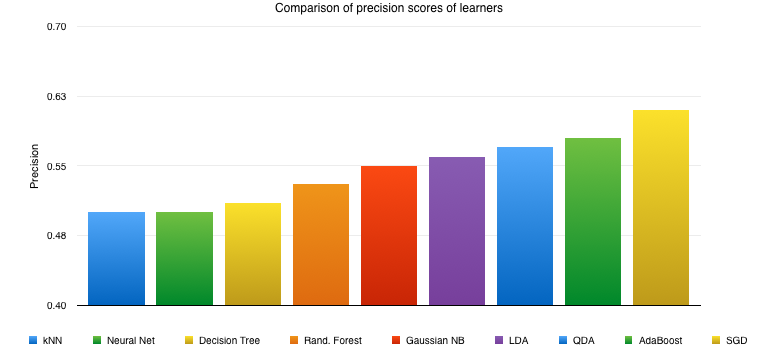
\includegraphics[width=\textwidth]{learner_comparison}
	\caption{Comparison of precision scores of learners on dataset with missing data deleted and no oversampling performed.}
	\label{fig:learner_comp}
\end{figure*}

Figure~\ref{fig:learner_comp} shows the precision scores of the various methods discussed above. Results across the board were not particularly impressive compared to the random baseline of 0.333, ranging from 0.49 to 0.61. k-Nearest Neigbor and Neural Net performed the worst. The highest-performing algorithm was the Support Vector Machine (SGD), followed by AdaBoost.

\begin{figure}[htpb]
	\centering
	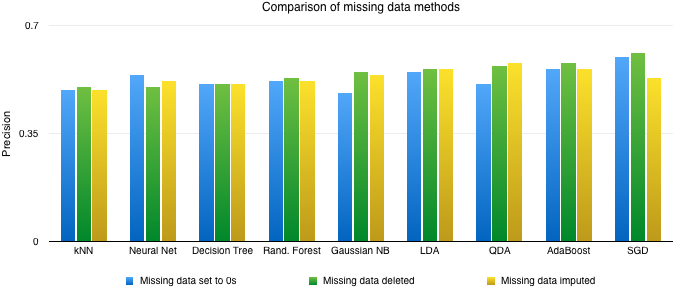
\includegraphics[width=0.5\textwidth]{missing_data_comparison}
	\caption{Comparison of missing data methods via precision scores of learners.}
	\label{fig:missing_data_comp}
\end{figure}

A comparison of the various methods to handle missing data is presented in figure~\ref{fig:missing_data_comp}, with precision scores from all learners shown. Generally, missing data set to its own category performed worse than both deletion and imputation, which each performed equally on average. There are some exceptions to this trend, specifically with Neural Networks, Gaussian Naive Bayes, and SVM, where one method is slightly better or worse than the other two.

\begin{figure}[htpb]
	\centering
	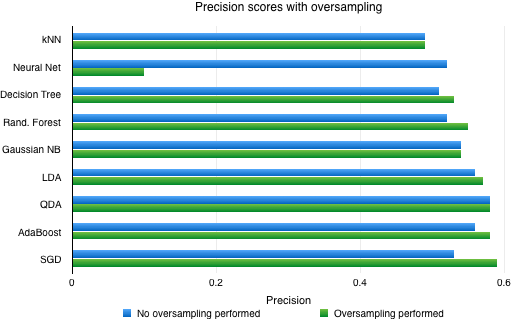
\includegraphics[width=0.5\textwidth]{oversampling_comparison}
	\caption{Precision scores of learners with and without oversampling of under-represented target classes, on a dataset with missing data deleted.}
	\label{fig:oversampling_comp}
\end{figure}

Figure~\ref{fig:oversampling_comp} shows the effect of oversampling on precision scores of the various learners. On average, oversampling of under-represented target classes performed equal to or better than not oversampling, particularly with SGD where the score improved by 0.6. One significant outlier was the Neural Network algorithm, where oversampling performed much worse than not oversampling.

\begin{figure}[htpb]
	\centering
	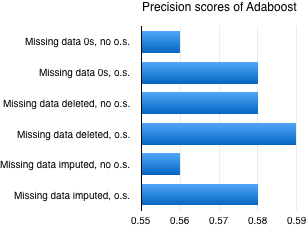
\includegraphics[width=0.5\textwidth,scale=0.75]{adaboost}
	\caption{Precision scores of Adaboost learner for various data pre-processing combinations.}
	\label{fig:adaboost}
\end{figure}

The combinations of missing data methods and oversampling are presented in figure~\ref{fig:adaboost} with precision scores using the Adaboost algorithm. Results were very similar across the combinations, with scores only ranging from 0.56 to 0.59. Deleting missing data and oversampling performed the best at 0.59, while not performing oversampling and either imputing missing data or setting it to a separate category performed the worst at 0.56.

\begin{figure}[htpb]
	\centering
	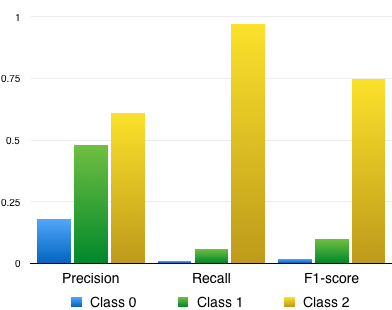
\includegraphics[width=0.5\textwidth]{full_results}
	\caption{Sample results of SGD learner on dataset with imputed missing data.}
	\label{fig:full_results}
\end{figure}

Precision, recall, and f1-score metrics for the three target classes using a sample learner (Support Vector Machines) with imputation for missing data is shown in figure~\ref{fig:full_results}. Although average values for each metric seem relatively stable (0.53 for precision, 0.60 for recall and 0.48 for f1-score), looking deeper at the breakdown of class values show an imbalance, with class 1 performing much worse than class 2, and class 2 performing much worse than class 3.

\begin{figure}[htpb]
	\centering
	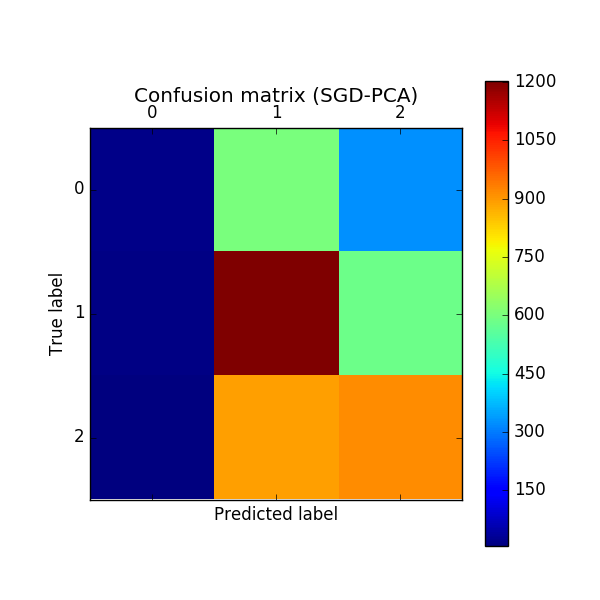
\includegraphics[width=0.5\textwidth]{confmatrix_sgd-pca}
	\caption{Confusion matrix of SGD learner with PCA on dataset with deleted missing data.}
	\label{fig:sgd_pca_results}
\end{figure}

The best results of applying PCA before SVM classification are shown below~\ref{fig:sgd_pca_results}. We found an optimal performance with keeping the 32 principal components. While the overall f1-score was significantly worse with feature selection, it did improve the precision and recall on class 0 (.41 f1-score for class 0, .35 f1-score for class 1, .46 f1-score for class 2). For each class, SVM predicted the correct class more than any other class. ANOVA produced similar but less successful results and as such the results are not shown here.

\begin{figure}[htpb]
	\centering
	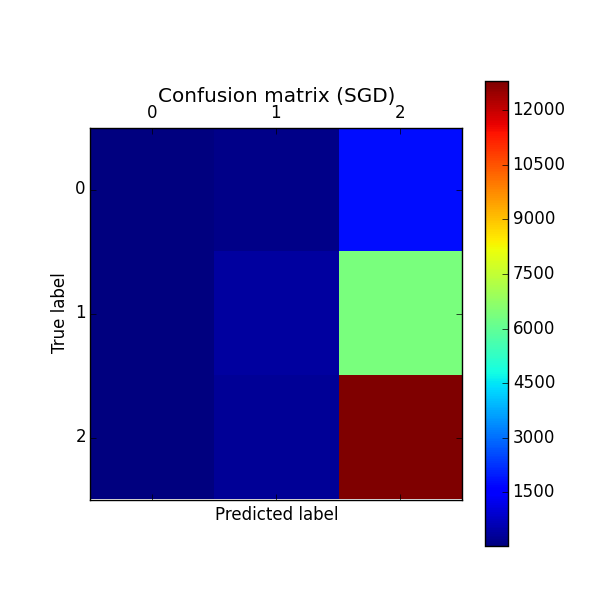
\includegraphics[width=0.5\textwidth]{full_results_confmatrix_SGD_md=imputed_ns=all_nc=3_os=f_test}
	\caption{Confusion matrix of SGD learner on dataset with imputed missing data.}
	\label{fig:full_results_cm}
\end{figure}

The confusion matrix for figure~\ref{fig:full_results} is shown in figure~\ref{fig:full_results_cm}. This figure displays that the majority of predictions are for class 2, even when the true class is 0 or 1. There are relatively much fewer predictions of class 0 or 1.

\section{Discussion}

Performance of complex classifiers was better than the baseline classifier because of efficient decision boundary conditions which prevents the overfitting problem as shown in Figure~\ref{fig:learner_comp}. Dataset used herein had class imbalance and missing data problem which was observe to effect the performance of the classifiers. Different methods of handling the missing data and class imbalance was utilized. However, it was observed that the deletion method of missing data performed better than the substitution method. Detailed study is required before utilizing any substitution method because of the nature of missing data i.e. MCAR or MAR, which was beyond the scope of this project. However, the oversampling method to resolve the class imbalance problem increased the performance of classifier as shown in Figure~\ref{fig:adaboost}. It can be observed that with six different combinations of missing data and class imbalance techniques, the results varied by only 3\%. So there may be some inherent anomalies in the dataset which is causing such poor performance of every technique. Most of the classifier performed better with the oversampling as shown in Figure~\ref{fig:oversampling_comp}. However, the class imbalance problem resulted in very low precision score of all the classifier for class 0. Figure~\ref{fig:full_results_cm} represents the confusion matrix of SGD classifier where the classifier was able to classify better class 1 and class 2 but was not able to classify class 0 properly due to the class imbalance problem. 

\section{Conclusion}

Dataset utilized for prediction of readmission rates consists of records from 130 U.S hospitals. Target prediction task was to determine the readmission rate of diabetic patients. Missing data and class imbalance problem with the dataset was handled using data substitution, data deletion methods for missing data and oversampling using SMOTE for class imbalance problem. Feature selection method such as PCA and ANOVA was also used for feature reduction and feature selection. Data deletion method was observed to perform better than data substitution method. However, the oversampling of the dataset using SMOT enhanced the performance of some classifiers but performed worst with some of the classifiers. Feature selection was observed to perform even worst and was not utilized for the classifiers herein. Literature with the diabetic databases suggested better performance of neural network, however the same was not observed with this dataset. Neural network performed worse than some of the baseline classifiers for oversampling method but performed good without the oversampling methods for class imbalance problems. Complex classifiers such as SGD and Adaboost was observed to perform better than baseline classifier such as Naïve Bayes, LDA, k-Nearest Neighbour etc. with the exception of Neural Network.

\section{Future Work}

Precision score for all the classifiers was very low for class 0 compared to other classes due to class imbalance problem. Class imbalance problem with the dataset seems to degrade the performance of classifier very heavily. Oversampling method such as SMOT was utilized to deal with this problem but was not observe to perform so well. Advance methods for class imbalance problem can be utilized in future to improve the performance of the classifiers. Otherwise more data can be collected to achieve higher performance. More advance classifier such as Recurrent Neural Network can be utilized in future to observe the performance. Missing data imputation using model based approach was observed to perform worse than the deletion method of missing data. More detailed study of the missing data including the reason of missing data (MCAR, MAR) can be performed to get insight into the actual reason of missing data and utilizing proper approach for handling those data.

\appendices
\section{Statement of Contributions}
This report is a joint contribution of all the team members. Data Imputation and Data Imbalance problem was done by Ashish. Jonathan did the algorithms for machine learning classification including neural network. Feature selection and SVM was done by Charlie.

We hereby state that all work presented in this report is that of the authors.

\printbibliography

\begin{IEEEbiography}[{\includegraphics[width=1in,height=1.25in,clip,keepaspectratio]{picture}}]{John Doe}
\blindtext
\end{IEEEbiography}

\end{document}